%!TEX root = main.tex

\section{Symmetric functions}

\subsection{Introduction}

	Let $G = \{x_1,x_2,\ldots,\}$ be a countably infinite abelian group.\\ 
	Consider the group action induced by the set of permutations of $\N$ on the set of monomials $x_{i_1}^{\alpha_{i_1}}\cdots x_{i_k}^{\alpha_{i_k}}$. For example,
	if $\sigma = (1,2)$ and $m = x_1^2x_2x_4^3$, then $\sigma(m) = x_1x_2^2x_4^3$.
	$\sigma$ thus acts on $\Q[x_1,\ldots,]$ by extending this linearly. A function $f$ is said to be symmetric if $\sigma(f) = f$ for all $\sigma$. The collection of homogeneous degree $d$ symmetric functions (with the zero polynomial) forms a vector space over $\Q$.

	\begin{fex}
		The unique symmetric function (up to scaling) of degree $1$ is $f = \sum_{i \ge 1} x_i$.\\
		For $d=2$, we get $\sum_{i<j} x_ix_j$ and $\sum_i x_i^2$ as a basis.
	\end{fex}

	Denote the vector space of $\Lambda_\Q^d$. It is not too difficult to show that $\dim(\Lambda_\Q^d) = p(d)$, the number of number-partitions of $d$.\\
	The basis of $\Lambda_\Q^d$ suggested by the above example is as follows. Let $\lambda = (\lambda_1,\ldots,\lambda_{\ell(\lambda)})$ be a partition of $d$ (denoted $\lambda \vdash d$). Define the monomial symmetric function
	\[ m_\lambda = \sum_{\text{symmetric}} x_1^{\lambda_1} x_2^{\lambda_2} \cdots x_k^{\lambda_k} = \sum \textbf{x}^\lambda. \]
	The ``symmetric'' means that we sum over all distinct ways to permute the exponents $\lambda_1,\ldots,\lambda_k$. The summation above is slightly strange, because we want to ensure that every monomial in $m_\lambda$ appears with coefficient $1$. $\{m_\lambda\}_{\lambda \vdash d}$ is a basis of $\Lambda_\Q^d$.

	\begin{question}
		\label{question: rowsum colsum}
		Given a matrix $M_{r \times k}$, on summing each row of $M$, we get a vector $\rowsum(M) = (r_1,\ldots,r_\ell)$ and on summing the columns we get a vector $\colsum(M) = (c_1,\ldots,c_k)$. When does there exist a 0-1 matrix $M$ such that $\rowsum(M)$ and $\colsum(M)$ are each equal to given vectors $(r_1,\ldots,r_\ell)$ and $(c_1,\ldots,c_k)$?
	\end{question}

	For starters, we clearly require $\sum r_i = \sum c_j \eqqcolon S$. Assume without loss of generality that $r_1 \ge \cdots \ge r_\ell$ and $c_1 \ge \cdots \ge c_k$ -- if a matrix for this exists, we can first reorder the rows to ensure the correct order of row sums, then reorder the columns. That is, we have two number partitions $\lambda = (r_1,\ldots,r_\ell)$ and $\mu = (c_1,\ldots,c_k)$ of $S$.\\
	We shall return to the problem later.\\


	Now, we define some partial orders on the set of number partitions.\\
	First, we consider an order that allows the comparison of number partitions of different numbers.
	\begin{fdef}[Young's order]
		Under \emph{Young's order}, given two number partitions $\lambda,\mu$, $\lambda \ple \mu$ iff the Ferrer diagram of $\lambda$ is contained in that of $\mu$.
	\end{fdef}
	Observe that under this order, two number partitions of the same number are \emph{not} comparable.\\

	Next, we define a total order over number partitions of a fixed number.
	\begin{fdef}[Lexicographic order]
		Fix some $d$ and two partitions $\lambda = (\lambda_1,\ldots,\lambda_k),\mu = (\mu_1,\ldots,\mu_\ell)$ of $d$. Under the \emph{lexicographic order}, we have $\lambda < \mu$ iff for some $r \le k$, $\lambda_r < \mu_r$ and $\lambda_i = \mu_i$ for all $i < r$.
	\end{fdef}

	% fubini polynomial: \sum_k S(n,k) k! x^k. (relevant to midsem question)

	Finally, we define a partial order over number partitions of a fixed number.
	\begin{fdef}[Dominance/Majorisation Order]
		\label{def: majorisation order}
		Fix some $d$ and two partitions $\lambda = (\lambda_1,\ldots,\lambda_{\ell(\lambda)}),\mu = (\mu_1,\ldots,\mu_{\ell(\mu)})$ of $d$. Padding zeros at the end of one of the partitions, assume that $\ell(\lambda) = \ell(\mu) \eqqcolon p$. Under the \emph{majorisation order}, we have $\lambda \ple \mu$ iff for $1 \le j \le p$,
		\[ \sum_{i=1}^j \lambda_i \le \sum_{i=1}^j \mu_i. \]
	\end{fdef}

	% A majorises B iff it can be written as a convex combination of B and its rearrangements (Birkhoff polytope related!)

\subsection{Elementary symmetric functions}

	We shall now see another basis of $\Lambda_\Q^d$. Consider the \emph{elementary symmetric functions}
	\[ e_{n} = m_{1^n} = \sum_{i_1 < i_2 < \cdots < i_n} x_{i_1} x_{i_2} \cdots x_{i_n}. \]
	Recall that $p(d)$ grows exponentially with $d$. Observe that if $f,g$ are symmetric functions, then $fg$ is also symmetric. For example,
	\[ m_1^2 = \left( \sum_i x_i \right)\left( \sum_i x_i \right) = m_2 + m_{1,1}. \]
	Multiplying increases the degree as well, which is the number the partition corresponds to. As another example,
	\[ m_2 m_1 = m_3 + m_{2,1}. \]
	For $\lambda \vdash d$ with $\lambda = \lambda_1,\cdots,\lambda_\ell$, where $\ell \ge 2$ (we have already looked at the case where $\lambda = d$), define
	\[ e_\lambda = \prod_{i=1}^\ell e_{\lambda_i}. \]
	For example,
	\begin{align*}
		e_3 &= m_{1^3} = \sum_{i < j < k} x_i x_j x_k \text{ and} \\
		e_{2,1} &= e_2e_1 = \left(\sum_{i < j} x_i x_j\right) \left(\sum_k x_k\right) = 3m_{1,1,1} + m_{2,1}.
	\end{align*}
	We claim that $\{e_\lambda : \lambda \vdash d\}$ is a basis of the set of symmetric functions.\\
	In the case of $d = 4$, we have
	\begin{align*}
		e_4 &= 1 m_{1^4} \\
		e_{3,1} &= 4m_{1^4} + 1m_{2,1,1} \\
		e_{2,2} &= 6m_{1^4} + 2m_{2,1,1} + 1m_{2,2} \\
		e_{2,1,1} &= 12m_{1^4} + 5m_{2,1,1} + 2m_{2,2} + 1m_{3,1} \\
		e_{1^4} &= 24m_{1^4} + 12m_{2,1,1} + 6m_{2,2} + 4m_{3,1} + 1m_{4}.
	\end{align*}

	As the coefficients seem to be non-negative and integral, one can ask for a combinatorial interpretation. If
	\[ e_\lambda = \sum_{\mu \vdash d} M_{\lambda\mu} m_\mu, \]
	what is $M_{\lambda\mu}$?

	\begin{ftheo}
		\label{theo: sol to rowsum colsum}
		Let $\lambda,\mu \vdash d$. Then, $M_{\lambda\mu}$ is the number of $\ell(\lambda) \times \ell(\mu)$ $0,1$-matrices $A$ with $\rowsum(A) = \lambda$ and $\colsum(A) = \mu$.
	\end{ftheo}
	Recall \Cref{question: rowsum colsum}.
	\begin{proof}
		Let $\ell(\lambda) = r, \ell(\mu) = k$.\\
		Consider the $r \times k$ matrix
		\[ \begin{bmatrix} x_1 & x_2 & \cdots \\ x_1 & x_2 & \cdots \\ \vdots & \vdots & \ddots \end{bmatrix}. \]
		Choose a $0,1$ vector with $\lambda_i$ $1$s and paste it in in $M$ at the $i$th row. The coefficient of $x_1^{\mu_1} x_2^{\mu_2} \cdots x_k^{\mu_k}$ in $\prod_i e_{\lambda_i}$ is given by choosing for each $i \in [r]$ a set of indices in $[k]$ such that
	\end{proof}
	
	Consider the $p(d) \times p(d)$ matrix $M$ with the ${\lambda,\mu}$th entry equal to the $M_{\lambda\mu}$ that we defined earlier.
	
	\begin{fcor}
		$M$ is symmetric.
	\end{fcor}
	This follows immediately from \Cref{theo: sol to rowsum colsum} upon taking the transpose of any matrix.

	\begin{ftheo}[Gale-Ryser]
		\label{gale-ryser}
		Let $\lambda,\mu \vdash d$. There exists a $0,1$-matrix $A$ with $\rowsum(A) = \lambda,\colsum(A) = \mu$ iff $\lambda \ple \mu^*$ under the \hyperref[def: majorisation order]{majorisation order}.
	\end{ftheo}

	Here, $\lambda^*$ is the \emph{conjugate} partition of $\lambda$, which is such that its Ferrer diagram is the transpose of that of $\lambda$. More precisely,
	\[ (\lambda^*)_i = \left| \left\{ j : \lambda_j \ge i \right\} \right|. \]
	For a proof of the above, one can see \href{http://www.math.iitb.ac.in/~krishnan/phd-2022/krause_gale_ryser.pdf}{this link}. Note that the notation used here swaps our definitions of row sum and column sum. % someone told Manfred Krause the problem and in a week, he had a simple solution!
	% the proof strategy is to start with \lambda^* and perturb it slightly until we get to \mu, and build a 0-1 matrix on the way.

	%%%% ***TODO*** : GALE RYSER

	% \begin{proof}
	% 	% \mu = colsum = q, \lambda = rowsum = p
	% 	The forward direction of the theorem is straightforward and we omit the proof.\\ % keep shifting 1s to the left to get larger colsums without changing rowsum, finally you just end up with p^* (which dominates colsum(A) = q)
		% Let $\mu = (m_1,\ldots,\mu_\ell)$. Let $r \pge q$ be arbitrary. Consider the minimum $i,j$ such that $r_i > q_i$ and $r_j < q_j$. % subtract 1 from r_i and add 1 at r_j. r' \ge q as well. Clearly, |r' - q| < |r - q| (2 norm). repeating this over and over, we finally just get q. Now, consider the matrix starting with Ferrer diagram of \lambda^*. Now, r_i > q_i \ge q_j > r_j. Choose the smallest h such that a_{h i} = 1 and a_{h j} = 0. Swap these two. Repeat over and over.
	% \end{proof}

	\begin{prop}
		Given partitions $\lambda,\mu \vdash d$, $\lambda \ple \mu^*$ iff $\mu \ple \lambda^*$.
	\end{prop}
	\begin{proof}
		% ****TODO****
		% We shall show that if $\lambda \ple \mu$, then $\mu^* \ple \lambda^*$. Fix some $t$. Note that
		% \[ \sum_{i=1}^t \min\{\lambda_i,t\} = \sum_{i=1}^t \min\{\lambda_i^*,t\} \]
		% and also that
		% \[ d = \sum_{i=1}^t \min\{\lambda_i,t\} + \sum_{i=1}^t (\lambda_i-t)_+ + \sum_{i=1}^t (\lambda_i^*-t)_+, \]
		% where $r_+ = r$ if $r \ge 0$ and $0$ otherwise. Consequently,
		% \[ d = \sum_{i=1}^t \lambda_i^* + \sum_{i=1}^t (\lambda_i-t)_+. \]
		% So, it suffices to show that
		% \[ \sum_{i=1}^t (\lambda_i-t)_+ \le \sum_{i=1}^t (\mu_i-t)_+. \]
	\end{proof}
	
	Let us now return to the question of whether the $e_\lambda$ form a basis of $\Lambda_{\Q}^d$. We would like to show that $M$ is invertible.

	\begin{enumerate}
		\item First, suppose that the partitions that index the and the rows lexicographically, starting with the partition $1^n$ and ending with $n$. Totally order the columns as $\lambda^{(1)},\lambda^{(2)},\ldots,\lambda^{(p(d))}$ such that it is compatible with majorisation -- if $\mu \pge \theta$, then $\mu \ge \theta$ (in our new order), and the reverse conjugate order is also compatible with majorisation. It turns out that the reverse lexicographic order satisfies this. 
		\item Show that this new matrix is upper triangular. To prove this, show that the lexicographic order is a topological sorting of the majorisation partial order.
		\item Argue that all the diagonal elements of this matrix are nonzero (in fact, they are $1$). This amounts to showing that the diagonal elements correspond to partition pairs of the form $(\lambda,\lambda^*)$.
	\end{enumerate}

	\begin{prop}
		\label{lem: invertible M 2}
		The lexicographic order is a topological sorting of the majorisation partial order.
	\end{prop}
	% \begin{exercise}
	% 	Prove the above.
	% \end{exercise}
	\begin{proof}
		This amounts to showing that if $\lambda \pge \mu$, then $\lambda \ge_{\text{lex}} \mu$. Let $t$ be the first index where $\lambda_t \ne \mu_t$. Then, $\sum_{i=1}^t \lambda_i \ge \sum_{i=1}^t \mu_i$, and since $\lambda_i = \mu_i$ for $i < t$, this implies that $\lambda_t \ge \mu_t$, proving the claim. 
	\end{proof}

	\begin{corollary}
		The lexicographic order is compatible with majorisation, and so is its reverse conjugate.
	\end{corollary}
	\begin{proof}
		The first part is precisely what we showed in the previous proposition. For the second part, we have that if $\lambda \pge \mu$, then $\mu^* \pge \lambda^*$, so $\lambda^* \ge_{\text{revlex}} \mu^*$. Indeed, if $r$ is the first index where $\lambda_r,\mu_r$ differ, we have
		\[ \lambda_r = \sum_{i=1}^r \lambda_i \ge \sum_{i=1}^r \mu_i = \mu_r. \qedhere \]
	\end{proof}

	\begin{fcor}
		\label{theo: eL form basis}
		$M$ is invertible and has an integral inverse. Consequently, $\{e_\lambda\}_{\lambda \vdash d}$ is a basis of $\Lambda_\Q^d$.
	\end{fcor}
	\begin{proof}
		By \Cref{lem: invertible M 2,gale-ryser}, $M$ is upper triangular. Further, $M_{\lambda\lambda^*} = 1$ for all $\lambda$. Therefore, $M$ is invertible. As it has determinant $1$, it has an integral inverse.
	\end{proof}

	\begin{fdef}[Algebraic independence over $\R$]
		Let $\A$ be an algebra. $\alpha_1,\alpha_2,\ldots\in \A$ are said to be \emph{algebraically independent} over $\R$ if there exists no polynomial $f$ with coefficents in $\R$ such that $\restr{f(y_1,\ldots)}{y_i = \alpha_i} = 0$.
	\end{fdef}

	Recall that $\Lambda_\Q^d$ is an algebra over $\R$.

	\begin{fcor}
		\label{cor: en algebraic indep}
		$\{e_n\}_{n \ge 1}$ are algebraically independent.
	\end{fcor}
	\begin{proof}
		Suppose instead that there exists a polynomial $f(y_1,\ldots)$ such that $\restr{f(y_1,\ldots)}{y_i = e_i} = 0$.\\
		Because monomials of different degree do not interact, we may assume that $\deg(\restr{m_j}{y_i = e_i}) = d$ for all monomials $m_j$ for some $d$. Therefore,
		\[ \restr{f(y_1,\ldots)}{y_i = e_i} = \sum_{\lambda \vdash d} c_\lambda e_\lambda \]
		where some $c_\lambda \ne 0$. This immediately contradicts \Cref{theo: eL form basis}, which says that the $\{e_\lambda\}_{\lambda \vdash d}$ are linearly independent.
	\end{proof}

	Linear independence implies algebraically independence!\\

	Consider the following, where we look at the products of finitely many terms on the left.
	\[ \prod_{i,j \ge 1} \left( 1 + x_iy_j \right). \]
	This gives meaningful terms when we choose finitely many terms of the form $x_iy_j$ and $1$ from the rest. Now, any such choice can be though of as an $r \times s$ $0,1$-matrix $A$, where $A_{ij} = 1$ if we choose $x_i y_j$ and $0$ otherwise. The contribution of this matrix $A$ is just $x^{\rowsum(A)} y^{\colsum(A)}$! Therefore,
	\begin{align}
		\prod_{i,j \ge 1} \left( 1 + x_i y_j \right) &= \sum_{\text{$A$ finite $0,1$-matrix}} x^{\rowsum(A)} y^{\colsum(A)} \nonumber \\
			&= \sum_{d \ge 0} \sum_{\lambda,\mu \vdash d} M_{\lambda\mu} m_\lambda(x) m_\mu(y) \nonumber \\
		\prod_{i,j \ge 1} \left(1 + x_iy_j\right)  &= \sum_{d \ge 0} \sum_{\lambda \vdash d} m_\lambda(x) e_\lambda(y).
	\end{align}

	\begin{prop}
		\label{eqn: prod 1 p xi yj}
		\[ \prod_{i,j \ge 1} (1+x_iy_j) = \sum_{\lambda \vdash d} m_\lambda(x) e_\lambda(y) \]
	\end{prop}

\subsection{Homogenous symmetric functions}

	Define a new class of symmetric functions, known as the \emph{complete homogenous symmetric functions}, by
	\[ h_n = \sum_{\mu \vdash n} m_\mu \]
	and for $\lambda = (\lambda_1,\ldots,\lambda_\ell) \vdash d$,
	\[ h_\lambda = \prod_{i=1}^{\ell} h_{\lambda_i}. \]
	For example,
	\begin{align*}
		h_2 &= m_2 + m_{1,1} \\
		h_{1,1} &= (m_1)^2 = m_2 + 2m_{1,1} \\
		h_3 &= m_3 + m_{2,1} + m_{1,1,1} \\
		h_{2,1} &= (m_2 + m_{1,1}) m_1 = m_3 + 2m_{2,1} + 3m_{1,1,1} \\
		h_{1,1,1} &= m_1^3 = m_3 + 3m_{2,1} + 6m_{1,1,1}.
	\end{align*}

	As in the $e_\lambda$, is it true that $h_\lambda$ is a non-negative integer combination of the $m_\mu$?
	\begin{flem}
		Let $\lambda \vdash d$. If
		\[ h_\lambda = \sum_{\mu \vdash d} N_{\lambda\mu} m_\mu, \]
		then $N_{\lambda\mu}$ is the number of $\N$-matrices $A$ with $\rowsum(A) = \lambda, \colsum(A) = \mu$.
	\end{flem}
	\begin{proof}
		As before, we shall establish a bijection between the set of described matrices and the terms in the product that contribute to $m_\mu$ (each way of taking products).\\
		Let $\lambda = \lambda_1,\ldots,\lambda_\ell$ and $\mu = \mu_1,\ldots,\mu_k$. Given a way of taking products, taking $m_{\theta_i} = \sum x^{\theta_i}$ from $h_{\lambda_i}$, consider the $\ell \times k$ matrix that assigns the power of $x_r$ to the $(r,i)$th entry.\\ 
		Because $h_n = \sum_{\theta \vdash n} m_\theta$, we now have the advantage of choosing any entries in the $r$th row, as long as the sum is $\lambda_r$.
	\end{proof}

	% The counterpart of the Gale-Ryser Theorem here is as follows.

	\begin{prop}
	% \begin{exercise}
		Prove that $N_{\lambda\mu} \ne 0$ for any $\lambda,\mu \vdash d$. That is, show that there always exists an $\N$-matrix $A$ such that $\rowsum(A) = \lambda,\colsum(A) = \mu$.\\
		Try to write a program that takes $\lambda,\mu$ as input and outputs such a matrix.
	% \end{exercise}
	\end{prop}
	\begin{proof}
		We prove it using strong induction on $d$. The base case where $d = 1$ is trivial. Otherwise, fill the first $(1,1)$ element of the matrix with $\min\{\lambda_1,\mu_1\}$. Assume that $\lambda_1 \ge \mu_1$. Now, we only need to fill the submatrix omitting the first column of a matrix with elements such that the row-sum is $(\lambda_1-\mu_1,\lambda_2,\ldots)$ and the column-sum is $(\mu_2,\mu_3,\ldots)$. Such a filling exists by the inductive hypothesis.
	\end{proof}

	It turns out, however, that the problem of determining $N_{\lambda\mu}$ is $\#\mathsf{P}$-complete.\\ % prof wasn't sure though.
	The next natural question to ask is: are the $(h_\lambda)$ a basis as well?\\
	Before moving to this, let us quickly look at analogues of \Cref{eqn: prod 1 p xi yj}. We jave
	\begin{align}
		\prod_{i,j \ge 1} \frac{1}{1-x_iy_j} &= \prod_{i,j \ge 1} \left(1 + (x_iy_j) + (x_iy_j)^2 + \cdots\right) \nonumber \\
			&= \sum_{\text{$A$ finite $\N$-matrix}} x^{\rowsum(A)} y^{\colsum(A)} \nonumber \\
			&= \sum_d \sum_{\lambda,\mu \vdash d} N_{\lambda\mu} m_\lambda(x) m_\mu(y) \nonumber \\
		\prod_{i,j \ge 1} \frac{1}{1-x_iy_j} &= \sum_d \sum_{\lambda \vdash d} m_\lambda(x) h_\lambda(y). \label{eqn: prod 1 m xi yj}
	\end{align}

	Recall that $\Lambda_{\Q}$ is generated by $\{e_n\}_{n \ge 1}$.

	\begin{ftheo}
		\label{theo: h basis}
		Consider the algebra homomorphism $\omega : \Lambda_\Q \to \Lambda_\Q$ defined by $\omega(e_n) = h_n$ for all $n$, so $\omega(e_\lambda) = h_\lambda$.\\
		$\omega$ is an involution. In particular, $(h_\lambda)_{\lambda \vdash d}$ form a basis of $\Lambda_\Q^d$.
	\end{ftheo}
	\begin{proof}
		Let $E(t) = \sum_{n \ge 0} e_n t^n$ be the ogf of the $e_i$, and similarly $H(t) = \sum_{n \ge 0} h_n t^n$. By \Cref{eqn: prod 1 m xi yj,eqn: prod 1 p xi yj}, setting $x = (t,0,0,\ldots)$ and noting that $m_\lambda(x) \ne 0$ iff $\lambda$ is $n$, we have that
		\begin{align*}
			E(t) &= \prod_{i \ge 1} (1+x_it) \\
			H(t) &= \prod_{i \ge 1} \frac{1}{(1-x_it)}.
		\end{align*}
		% \begin{exercise}
		% 	Prove the above.
		% \end{exercise}
		That is, $H(t) E(-t) = 1$. Therefore, for $r > 0$,
		\[ \sum_{0 \le k \le r} (-1)^{r-k} e_k h_{r-k} = 0. \]
		Now, let us prove by induction that $\omega(h_i) = e_i$. The base case, $n = 1$, is trivial since $e_1 = h_1$. Using the above equation for $r = n$, assuming that $\omega(h_k) = e_k$ for $k < n$, we get
		\begin{align*}
			0 &= \omega\left(\sum_{0 \le k \le n} (-1)^{n-k} e_k h_{n-k}\right) \\
				&= \sum_{0 \le k \le n} (-1)^{n-k} h_k \omega(h_{n-k}) \\
				&= (-1)^{n}\omega(h_n) + \sum_{1 \le k \le n} (-1)^{n-k} h_k e_{n-k} \\
				&= (-1)^{n}\omega(h_n) + (-1)^n \sum_{1 \le k \le n} (-1)^{k} h_k e_{n-k} \\
				&= (-1)^n \omega(h_n) - (-1)^n e_n + (-1)^n \sum_{0 \le k \le m} (-1)^k h_k e_{n-k} \\
			0 &= (-1)^n (\omega(h_n) - e_n).
		\end{align*}
		Therefore, $\omega$ is an involution. The second part of the theorem follows directly, because if the $\{h_\lambda\}_{\lambda \vdash d}$ were not linearly independent, then applying $\omega$ yields a violation to the linear independence of $\{e_\lambda\}_{\lambda \vdash d}$.
	\end{proof}

	\begin{remark}
		$\omega : \Lambda_\Q^d \to \Lambda_\Q^d$ is a linear transformation satisfying $\omega^2 - \Id = 0$. Therefore, the minimal polynomial of $\omega$ is $x^2 - 1 = 0$, and the characteristic polynomial of $\omega$ is $(x-1)^\alpha (x+1)^{p(d) - \alpha}$ for some $\alpha$. We shall figure out the value of $\alpha$ later, after \Cref{theo: p eigenbasis of omega}.
	\end{remark}

	% monomial symmetric functions is m_\lambda

\subsection{Power sum symmetric functions}

	Let us now look at one more class of symmetric functions, known as the \emph{power sum symmetric functions}. For $n > 0$, define
	\[ p_n = m_n = \sum_{i \ge 1} x_i^n. \]
	For $\lambda = (\lambda_1,\ldots,\lambda_\ell) \vdash d$, define
	\[ p_\lambda = \prod_{i=1}^\ell p_{\lambda_i}. \]

	Let
	\[ p_\lambda = \sum_{\mu \vdash d} R_{\lambda\mu} m_\mu. \]

	For example,
	\begin{align*}
		p_3 &= m_3 \\
		p_{2,1} &= m_3 + m_{2,1} \\
		p_{1,1,1} &= m_3 + 3m_{2,1} + 6m_{1^3}
	\end{align*}
	and
	\begin{align*}
		p_4 &= m_4 \\
		p_{3,1} &= m_4 + m_{3,1} \\
		p_{2,2} &= m_4 + 0m_{3,1} + 2m_{2,2} \\
		p_{2,1^2} &= m_4 + 2m_{3,1} + 2m_{2,2} + 2m_{2,1^2} \\
		p_{1^4} &= m_4 + 4m_{3,1} + 6m_{2,2} + 12m_{2,1^2} + 24m_{1^4}.
	\end{align*}
	It is obvious that $R_{\lambda\mu}$ is a non-negative integer for each $\lambda,\mu$. As before, is there some combinatorial interpretation of these coefficients?\\
	Let $\lambda = (\lambda_1,\ldots,\lambda_\ell)$ and $\mu = (\mu_1,\ldots,\mu_k)$. We want to find the number of ways to get $x_1^{\mu_1} x_2^{\mu_2} \cdots x_k^{\mu_k}$ on expanding
	\[ \left( \sum_{i_1 \ge 1} x_{i_1}^{\lambda_1} \right) \left( \sum_{i_2 \ge 1} x_{i_2}^{\lambda_2} \right) \cdots \left( \sum_{i_\ell \ge 1} x_{i_\ell}^{\lambda_\ell} \right). \]
	This number of ways is equal to the number of ordered partitions (sometimes called \emph{preferential arrangements}) $(S_1,\ldots,S_k)$ of $[\ell]$ such that for each $1 \le r \le k$,
	\[ \sum_{j \in S_r} \lambda_j = \mu_r.  \]

	\begin{ftheo}
		If $R_{\lambda\mu} > 0$, then $\mu \pge \lambda$.
	\end{ftheo}
	Note that unlike \nameref{gale-ryser}, this is not an iff statement.
	\begin{proof}
		Let $(S_1,\ldots,S_k)$ be an ordered partition of $[\ell]$ such that for each $1 \le r \le k$, $\sum_{j \in S_r} \lambda_j = \mu_r$. In particular, $\lambda_j \le \mu_r$ for any $j \in S_r$. \\
		Let $i \in S_{p_i}$ for each $i \in [\ell]$. Then, for any $1 \le r \le \ell$,
		\[ \sum_{i=1}^r \lambda_{i} \le \sum \mu_{p_i} \le \sum_{i=1}^r \mu_{i}, \]
		so $\mu \pge \lambda$.
	\end{proof}

	Therefore, the $p(d) \times p(d)$ matrix $R$ with rows and columns ordered reverse lexicographically is lower-triangular!\\
	Further, it is not too difficult to see that for $\lambda \vdash d$, $R_{\lambda\lambda} \ne 0$.
	
	% \begin{exercise}
		% Find a formula for $R_{\lambda\lambda}$.
	\begin{prop}
		Show that for $\lambda \vdash d$, if $\lambda = 1^{n_1}2^{n_2}\cdots d^{n_d}$,
		\[ R_{\lambda\lambda} = n_1! n_2! \cdots n_d!. \]
	\end{prop}
	% \end{exercise}
	\begin{proof}
		Suppose that $\lambda$ has $r$ parts. By the combinatorial interpretation of $R_{\lambda\lambda}$, we wish to find the number of preferential arrangements $(S_1,\ldots,S_r)$ of $[r]$ such that $\sum_{j \in S_k} \lambda_j = \lambda_k$. Since no $S_k$ can be empty, each $S_k$ must be a singleton, suppose that it contains the element $\sigma(k)$ (where $\sigma:[r]\to[r]$ is a permutation). The second condition gives that $\lambda_{\sigma(j)} = \lambda_j$ for each $j$. The number of such permutations is precisely
		\[ R_{\lambda\lambda} = n_1! n_2! \cdots n_d!. \]
	\end{proof}

	\begin{fcor}
		$\{p_\lambda\}_{\lambda \vdash d}$ is a basis of $\Lambda_\Q^d$.
	\end{fcor}

	% cool result: *complex* matrices A and A^\top are conjugate!
	Recall that two permutations in $\mathfrak{S}_d$ are conjugate iff they have the same cycle type, so a conjugacy class can be determined (``indexed'') by a partition of $[d]$. For $\lambda \vdash d$, define $z_\lambda$ by
	\[ \frac{d!}{z_\lambda} = \text{size of conjugacy class of $\mathfrak{S}_d$ indexed by $\lambda$}. \]

	Recall \Cref{eqn: prod 1 m xi yj,eqn: prod 1 p xi yj}.

	\begin{prop}
		\label{prod 1 m xi yj pLpL}
		\[ \prod_{i,j \ge 1} \frac{1}{1-x_iy_j} = \sum_{d \ge 0} \sum_{\lambda \vdash d} \frac{1}{z_\lambda} p_\lambda(x) p_\lambda(y). \]
	\end{prop}
	\begin{proof}
		We have
		\begin{align*}
			\log \left( \prod_{i,j \ge 1} \frac{1}{1-x_iy_j} \right) &= \sum_{i,j \ge 1} \log\left( \frac{1}{1-x_iy_j} \right) \\
				&= \sum_{i,j \ge 1} \sum_{n \ge 1} \frac{(x_iy_j)^n}{n} \\
				&= \sum_{n \ge 1} \frac{1}{n} \sum_{i,j \ge 1} (x_iy_j)^n \\
				&= \sum_{n \ge 1} \frac{1}{n} p_n(x)p_n(y).
		\end{align*}
		Now, we shall use the permutation formula \Cref{ec2: egf sum over perms}. Set $f_n = p_n(x) p_n(y)$. Then, the corresponding $g_n$ in the formula is given by
		\[ g_n = \sum_{\lambda \vdash n} \left( \frac{n!}{z_\lambda} \right) \cdot p_\lambda(x) p_\lambda(y). \]
		Therefore, setting $x = 1$ in the permutation formula, we get
		\begin{align*}
			\prod_{i,j \ge 1} \frac{1}{1-x_iy_j} &= \exp \left( \sum_{n \ge 1} \frac{1}{n} p_n(x) p_n(y) \right) \\
				&= \exp\left( \sum_{n\ge 1} \frac{1}{n} f_n \right) \\
				&= \sum_{n \ge 0} \frac{g_n}{n!} = \sum_{n \ge 0} \sum_{\lambda \vdash n} \frac{1}{z_\lambda} p_\lambda(x) p_\lambda(y). \qedhere
		\end{align*}
	\end{proof}

	We can also get an explicit formula for $z_\lambda$. Let $c_\lambda = n!/z_\lambda$ be the size of conjugacy class of $\mathfrak{S}_d$ indexed by $\lambda$. Let $\lambda = 1^{m_1} 2^{m_2} \cdots n^{m_n}$, where $m_i \ge 0$ is the multiplicity of $i$ in $\lambda$. Clearly, $\sum_i i m_i = n$. Any permutation with cycle type $\lambda$ can be attained by taking a permutation in $\mathfrak{S}_n$, then grouping together the $\sum_{i \le r} i m_i + j + 1$ to $\sum_{i \le r} i m_i + j + r$ elements in a cycle of size $r$ for $0 \le j \le m_r-1$. Further, each permutation is overcounted (repeated) precisely $\prod_{i \ge 1} i^{m_i} m_i!$ times, so
	\[ c_\lambda = \frac{n!}{\prod_{i \ge 1} i^{m_i} m_i!} = \frac{n!}{z_\lambda}. \]
	% z_\lambda is interesting because it studies some stabilizer stuff

	% Setting $y_1 = t$ and everything else as $0$ in the previous proposition, we get the following.
	\begin{corollary}
		\[ h_n = \sum_{\lambda \vdash n} \frac{1}{z_\lambda} p_\lambda. \]
	\end{corollary}
	\begin{proof}
		Set $y_1 = t$ and everything else as $0$ in the previous proposition. Then,
		\[ \sum_{d \ge 1} h_d t^d = \prod_{i \ge 1} \frac{1}{1-tx_i} = \sum_d \left(\sum_{\lambda \vdash d} \frac{1}{z_\lambda} p_\lambda(x)\right) t^d. \]
		Matching the coefficients of $t^d$ completes the proof.
	\end{proof}

	\begin{prop}
		For any $\pi \in \mathfrak{S}_n$ with cycle type $\lambda$, setting $\epsilon_\lambda = \sign(\pi)$,
		\[ \prod_{i,j \ge 1} (1+x_iy_j) = \sum_{d \ge 0} \sum_{\lambda \vdash d} \frac{\epsilon_\lambda}{z_\lambda} p_\lambda(x) p_\lambda(y), \]
	\end{prop}
	% \begin{exercise}
		% Show that
		% \[ \prod_{i,j \ge 1} (1+x_iy_j) = \sum_{d \ge 0} \sum_{\lambda \vdash d} \frac{\epsilon_\lambda}{z_\lambda} p_\lambda(x) p_\lambda(y), \]
		% where $\epsilon_\lambda = (-1)^{d - \ell(\lambda)} = \sign(\pi)$ for any $\pi \in \mathfrak{S}_n$ with cycle type $\lambda$.
	% \end{exercise}
	% 
	\begin{proof}
		The proof is largely similar to that of \Cref{prod 1 m xi yj pLpL}, with the only difference being that in the log expansion, we get an extra $\epsilon_\lambda$ term.
	\end{proof}

	\begin{corollary}
		\[ e_n = \sum_{\lambda \vdash n} \frac{\epsilon_\lambda}{z_\lambda} p_\lambda. \]
	\end{corollary}

	The following may be proved in precisely the same way as \Cref{cor: en algebraic indep}.
	\begin{fpor}
		$\{p_n\}_{n \ge 1}$ and $\{h_n\}_{n \ge 1}$ are algebraically independent families.
	\end{fpor}

	Recall the involution $\omega$ from \Cref{theo: h basis}. What is $\omega(p_n)$, or $\omega(p_\lambda)$ more generally?

	\begin{ftheo}
		\label{theo: p eigenbasis of omega}
		For all $\lambda \vdash d$, $\omega(p_\lambda) = \epsilon_\lambda p_\lambda$. Therefore, $\{p_\lambda\}_{\lambda \vdash d}$ forms an eigenbasis of $\omega$, with $p_\lambda$ having eigenvalue $\epsilon_\lambda$, and $\omega$ is diagonalisable.
	\end{ftheo}
	Therefore, with respect to the $\{p_\lambda\}_{\lambda \vdash d}$ basis, $\omega$ as a linear transformation is diagonal. This gives us an alternate proof that $\omega^2 = \Id$. Further, it gives that
	\[ \Charpoly(\omega) = (x-1)^{\alpha(d)} (x+1)^{p(d) - \alpha(d)}, \]
	where $\alpha(d)$ is the number of partitions $\lambda \vdash d$ such that $d - \ell(\lambda)$ is even.
	\begin{proof}
		We think of $\omega$ acting on $m_\lambda(x)$ while symmetric functions in the variables $y_1,y_2,\ldots$ are thought of as scalars. Recalling that $\omega(e_\lambda) = h_\lambda$,
		\begin{align*}
			\sum_{d}\sum_{\lambda \vdash d} \frac{1}{z_\lambda} p_\lambda(y) \omega(p_\lambda(x)) &= \omega \left( \prod_{i,j \ge 1} \frac{1}{1-x_iy_j} \right) \\
				&= \omega \left( \sum_{d \ge 0} \sum_{\lambda \vdash d} m_\lambda(y) h_\lambda(x) \right) \\
				&= \sum_{d \ge 0} \sum_{\lambda \vdash d} m_\lambda(y) e_\lambda(x) \\
				&= \prod_{i,j \ge 1} (1+x_iy_j) \\
				&= \sum_{d \ge 0} \sum_{\lambda \vdash d} \frac{\epsilon_\lambda}{z_\lambda} p_\lambda(x) p_\lambda(y).
		\end{align*}
		Matching the coefficients of $p_\lambda(y)$, we get $\omega(p_\lambda) = \epsilon_\lambda p_\lambda$.
	\end{proof}

\subsection{Dual bases}

	We now endow $\Lambda_\Q^d$ with a scalar product (a bilinear form over $\Q$) by
	\[ \langle m_\lambda , h_\mu \rangle = \delta_{\lambda\mu} = \begin{cases} 1, & \lambda = \mu, \\ 0, & \text{otherwise.} \end{cases} \]
	
	Given this inner product, one can ask for an orthogonal basis of $\Lambda_\Q^d$.

	\begin{fdef}[Dual basis]
		If $\{u_\lambda\}$ and $\{v_\mu\}$ are a pair of bases for $\Lambda_\Q^d$ (for all $d$), we say that they are \emph{dual pair} of bases if $\langle u_\lambda , v_\mu \rangle = \delta_{\lambda\mu}$.
	\end{fdef}

	\begin{ftheo}
		\label{theo: characterize dual basis}
		If $\{u_\lambda\}_{\lambda \vdash d}$ and $\{v_\mu\}_{\mu \vdash d}$ are a pair of bases of $\Lambda_\Q^d$, then they form a dual pair iff
		\[ \prod_{i,j \ge 1} \frac{1}{1-x_iy_j} = \sum_{d \ge 0} \sum_{\lambda \vdash d} u_\lambda(x) v_\lambda(y). \]
	\end{ftheo}
	\begin{proof}
		Let
		\[ m_\lambda = \sum_{\varphi \vdash d} A_{\lambda\varphi} u_\varphi \text{ and } h_\mu = \sum_{\theta \vdash d} B_{\mu\theta} v_\theta. \]
		By definition,
		\begin{align*}
			\delta_{\lambda\mu} &= \langle m_\lambda , h_\mu \rangle \\
				&= \left\langle \sum_{\varphi \vdash d} A_{\lambda\varphi} u_\varphi , \sum_{\theta \vdash d} B_{\mu\theta} v_\theta \right\rangle \\
				&= \sum_{\varphi,\theta} A_{\lambda\varphi} B_{\mu\theta} \langle u_\varphi , v_\theta \rangle.
		\end{align*}
		Defining the $p(d) \times p(d)$ matrix $T$ by $T_{\varphi\theta} = \langle u_\varphi , v_\theta \rangle$, the above gives that
		\[ I_{p(d)} = A T B^\top. \]

		Suppose that $\{u_\lambda\},\{v_\mu\}$ form a pair of dual basis, so $T = I_{p(d)}$, and $I = AB^\top  = A^\top B$. That is,
		\[ \delta_{\lambda\mu} = \sum_{\theta \vdash d} A_{\theta\lambda} B_{\theta\mu}. \]
		Now,
		\begin{align*}
			\prod_{i,j \ge 1} \frac{1}{1-x_iy_j} &= \sum_{d \ge 0} \sum_{\lambda \vdash d} m_\lambda(x) h_\lambda(y) \\
				&= \sum_{d \ge 0} \sum_{\lambda \vdash d} \left( \sum_{\varphi \vdash d} A_{\lambda\varphi} u_\varphi(x) \right) \left( \sum_{\theta \vdash d} A_{\lambda\theta} v_\theta(y) \right) \\
				&= \sum_{d \ge 0} \sum_{\varphi,\theta \vdash d} u_\varphi(x) v_\theta(y) \left( \sum_{\lambda \vdash d} A_{\lambda\varphi} B_{\lambda\theta} \right) \\
				&= \sum_{d \ge 0} \sum_{\varphi \vdash d} u_\varphi(x) v_\varphi(y),
		\end{align*}
		completing the forward direction of the proof.\\
		The entire argument is reversible, and we omit the details of checking this.
	\end{proof}

	% NOT DONE
	% \begin{exercise}
		% Complete the above proof.
	% \end{exercise}

	Recall that
	\[ \prod_{i,j \ge 1} \frac{1}{1-x_iy_j} = \sum_{d \ge 0} \sum_{\lambda \vdash d} \frac{1}{z_\lambda} p_\lambda(x) p_\lambda(y), \]
	so
	\[ \langle  p_\lambda , p_\mu \rangle = z_\lambda \delta_{\lambda\mu}. \]

	\begin{fcor}
		\phantom{pain}
		\begin{enumerate}
			\item $\{ p_\lambda \}_{\lambda \vdash d}$ is an orthogonal basis of $\Lambda_\Q^d$.
			\item $\{ p_\lambda/\sqrt{z_\lambda} \}_{\lambda \vdash d}$ is a self-dual basis of $\Lambda_\R^d$.
			\item $\{ p_\lambda \}_{\lambda \vdash d}$ and $\{p_\lambda/z_\lambda\}_{\lambda\vdash d}$ form a pair of dual bases of $\Lambda_\Q^d$.
		\end{enumerate}
	\end{fcor}

	The above also allows us to show properties of symmetry, non-negativity etc.

	\begin{fcor}
		Let $f,g \in \Lambda_\Q^d$. Then,
		\begin{enumerate}
			\item $\langle f,g\rangle = \langle g,f\rangle$.
			\item $\langle f,f\rangle \ge 0$, with equality iff $f = 0$.
		\end{enumerate}
	\end{fcor}
	\begin{proof}
		Let $f = \sum_{\lambda \vdash d} A_\lambda p_\lambda$ and $g = \sum_{\lambda \vdash d} B_\lambda p_\lambda$. 
		\begin{enumerate}
			\item We have
			\[ \langle f,g \rangle = \sum_{\lambda \vdash d} z_\lambda A_\lambda B_\lambda = \langle g,f\rangle. \]
			\item We have
			\[ \langle f,f\rangle = \sum_{\lambda \vdash d} z_\lambda A_\lambda^2, \]
			which is non-negative and equal to $0$ iff all $A_\lambda$ are $0$. \qedhere
		\end{enumerate}
	\end{proof}

	% \begin{exercise}
		Start with $\{m_\lambda\}_{\lambda\vdash d}$ and run Gram-Schmidt Orthogonalization. What is the output orthogonal basis?
	% \end{exercise}

\subsection{Schur symmetric functions}

	Now, let us define another basis (which will turn out to be orthogonal).\\

	Let $\lambda \vdash d$. Consider the Ferrer's diagram of $\lambda$. We shall fill the boxes with positive integers such that
	\begin{enumerate}
		\item each row is weakly increasing from left to right and
		\item all columns are strictly increasing.
	\end{enumerate}

	\begin{fex}
		For the partition $\lambda = (3,1)$ of $4$,
		\[
		\begin{ytableau}
			1 & 1 & 2 \\
			3
		\end{ytableau}
		\]
		is such a filling.
	\end{fex}
	Such a filling is called a \emph{semi-standard Young Tableau} (SSYT) of shape $\lambda$. Let $F$ be an SSYT. Let $F$ have $m_i$ occurrences of $i$ in it -- this yields a vector $(m_1,m_2,\ldots,)$, called the \emph{content} of $F$ and denoted $\content(F)$. Clearly, $\sum_i m_i = d$.\\
	Define
	\[ S_\lambda = \sum_{\text{SSYTs $F$ of shape $\lambda$}} x^{\content(F)} \]
	For example, when $\lambda = (2,1)$,
	\[ S_\lambda = m_{2,1} + 2 m_{1^3} \]

	\begin{ftheo}[Knuth-Bender]
		Let $d \ge 0$ and $\lambda \vdash d$. Then, $S_\lambda$ is a symmetric function.
	\end{ftheo}
	\begin{proof}
		Fix some content vector $(m_1,m_2,\ldots)$. Let $\mathcal{F}$ be the set of SSYTs $F$ of shape $\lambda$ with $\content(F) = (m_1,m_2,\ldots)$. Fix arbitrary $i$, and let $\mathcal{F}_i$ be the set of SSYTs $F$ of shape $\lambda$ with $\content(F) = (m_1,m_2,\ldots,m_{i-1},m_{i+1},m_i,m_{i+2},m_{i+3},\ldots)$ (the $i$th and $(i+1)$th coordinates are swapped).\\
		We shall demonstrate a bijection $\varphi_i$ between $\mathcal{F}$ and $\mathcal{F}_i$ -- this implies the result because $i$ is arbitrary (Why?).\\
		Let $F \in \mathcal{F}$. In a given column, there are four possibilities.
		\begin{enumerate}
			\item both $i$ and $i+1$ occurs -- in this case, there must be precisely one of each in the column and they are consecutive.
			\item neither $i$ not $i+1$ occur.
			\item only $i$ or only $i+1$ occur -- in this case, there is precisely one of it in the column.
		\end{enumerate}
		In the first two cases, we say that the occurences of $i,(i+1)$ are ``paired''. In the third case, we say that the occurence is free. Suppose that some row of $F$ has $a$ $i$s and $b$ $(i+1)$s. Note that these $(a+b)$ occurrences are consecutive! Showing this requires the fact that $F$ is an SSYT -- show that all paired $i$s are before free $i$s, then that all free $(i+1)$s are before paired $(i+1)$s.\\
		We then define $\varphi_i(F)$ to be that filling where this consecutive block of $(a+b)$ elements is changed to have $b$ $i$s then $a$ $(i+1)$s; the remainder of the diagram is left unchanged compared to $F$. Note that this filling is indeed in $\mathcal{F}_i$! $\varphi_i$ is also clearly a bijection since the same operations define an inverse function from $\mathcal{F}_i$ to $\mathcal{F}$.
	\end{proof}

	The $(S_\lambda)$ are known as the \emph{Schur symmetric functions}.\\
	Note that for any $n$, $S_n = h_n$ and $S_{1^n} = e_n$.\\
	Let us now try to show, as per usual, that the $(S_\lambda)$ form a basis of $\Lambda_\Q^d$. We have
	\begin{align*}
		S_3 &= m_{1^3} + m_{2,1} + m_3 \\
		S_{2,1} &= 2m_{1^3} + m_{2,1} \\
		S_{1^3} &= m_{1^3}.
	\end{align*}

	Let
	\begin{equation}
		\label{eqn: kostka}
		S_\lambda = \sum_{\mu \vdash d} K_{\lambda\mu} m_\mu.
	\end{equation}
	Here, the $K_{\lambda\mu}$ are known as the \emph{Kostka numbers}. By definition, $K_{\lambda\mu}$ is the number of SSYTs with shape $\lambda$ and content $\mu$. In a spirit much like \nameref{gale-ryser}, we shall show that $K$ is upper-triangular when we order both the rows and columns in the reverse-lexicographic order.

	\begin{ftheo}
		$K_{\lambda\mu}$ is nonzero if and only if $\lambda \pge \mu$ (under the majorisation partial order).
	\end{ftheo}
	\begin{proof}
		First, suppose that $K_{\lambda\mu} \ne 0$. Note that the $i$th row cannot have any element less than $i+1$. In particular, all the $i$s for $i\le k$ are contained in the first $k$ rows. This precisely says that $\sum_{i=1}^r \lambda_i \ge \sum_{i=1}^r \mu_i$, since the first term is the number of cells in the first $k$ rows and the second is the number of $i \le k$ in the first $k$ rows.\\
		For the converse, given $\lambda \ge \mu$, we must construct an SSYT with shape $\lambda$ and content $\mu$. We do so in the following manner. Having filled all the elements $<r$, fill the $r$th row with $r$s as long as there are filled cells in the corresponding cell one row above. After doing this, fill any remaining $r$s in the $(r-1)$th row as long as there are filled cells in the corresponding cell one row above. Repeat this until $\mu_r$ $r$s are filled up. Both row-increasingness and column-strictness are trivial, and the construction is well-defined because $\sum_{i=1}^r \lambda_i \ge \sum_{i=1}^r \mu_i$.
	\end{proof}

	\begin{exercise}
		Complete the above proof.
		% Show that if $\lambda \pge \mu$, then $K_{\lambda\mu} \ne 0$
	\end{exercise}

	Now, note that the diagonal entries of $K$ are equal to $1$ by an argument similar to that of the previous theorem.
	\begin{fcor}
		$(S_\lambda)_{\lambda \vdash d}$ forms a basis of $\Lambda_\Q^d$. 
	\end{fcor}

	Unfortunately, $K_{\lambda\mu}$ has no good formula in general. However, there are formulae in certain special cases.\\
	When $\mu = 1^d$, we wish to determine the number of SSYTs with shape $\lambda$ such that each element of $\{1,2,\ldots,d\}$ occurs precisely once.

	\begin{fdef}
		A \emph{Standard Young Tableau} (SYT) of shape $\lambda\vdash d$ is an SSYT of shape $\lambda$ where each element of $[d]$ occurs precisely once. The number of SYTs of shape $\lambda$ is denoted $f_\lambda = K_{\lambda,1^d}$.
	\end{fdef}
	Note that this implies that rows are strictly increasing. The number of SYTs of a given shape has some very neat formulae!

	\begin{ftheo}[Hook length formula]
		Given a cell $c$ in the Ferrer diagram of $\lambda \vdash n$, the \emph{hook} at cell $c$ consists of $c$, cells to the right of $c$, and cells below $c$. Denote by $h_c$ the size of the hook at $\lambda$. Then,
		\[ f_\lambda = \frac{n!}{\prod_{c \in \operatorname{cell}(\lambda)} h_c}. \]
	\end{ftheo}
	We do not prove the above. The original proof was due to Frame, Robinson, Thrall, and Wilf, Nijenhuis later gave an easier proof.\\
	Using the above, note in particular that the number of SYTs of shape $(n,n)$ is
	\[ f_{n,n} = \frac{1}{n+1} \binom{2n}{n}, \]
	the $n$th Catalan number $C_n$!

\subsection{The RSK algorithm}

	\begin{ftheo}
		Let $\lambda \vdash n$. Recall that $\mathfrak{S}_n$ has $p(n)$ distinct irreducible representations (up to isomorphism), indexed by the conjugacy classes of $\mathfrak{S}_n$. Further, the irreducible representation indexed by $\lambda$ has dimension $f_\lambda$.\\
		Consequently,
		\[ \sum_{\lambda \vdash n} f_\lambda^2 = n!. \]
	\end{ftheo}


	Let us give an alternate bijective proof of this.
	% \begin{proof}[RSK algorithm]
	We would like to come up with a bijection 
	\[ \varphi : \{(P,Q) : P,Q \text{ are SYTs of the same shape}\} \to \mathfrak{S}_n. \]
	We use the \emph{RSK algorithm}. We start with a finite matrix $M$ with non-negative integer entries. We encode this as a $2 \times r$ matrix, where $r$ is the sum of entries of $M$. To construct this matrix, we iterate through the entries of $M$ in row-major form, and insert the column $\begin{pmatrix} i \\ j \end{pmatrix}$ $M_{ij}$ many times. Let the first row of this matrix be $Q$ and the second be $P$.\\
	By definition, the lengths of both $P$ and $Q$ is the sum of entries of $M$. Because we are iterating through the entries in row-major order, $P$ is weakly increasing. For example, in the case where $M$ is a permutation matrix, $Q$ is just $1,2,\ldots,n$ and $P$ some permutation of $[n]$.\\
	Now, using this new $2 \times r$ matrix, we shall form an SSYT. The algorithm just repeats the following. Iterating through $[r]$, suppose we are at the $i$th entry.
	\begin{enumerate}
		\item If it is possible to add $P_i$ at the end of the first row, we append it.
		\item If this is not possible, we insert it in the first row at the earliest possible position, ``kicking out'' some other entry. We then try to insert this entry in the part of the filling below the first row, recursively in the exact same manner as just described.
		\item Insert $Q_i$ at an appropriate position in order to ensure that the shapes of the tableaux remain the same.
	\end{enumerate}

	\begin{fex}
		Suppose our initial matrix is
		\[
		\begin{pmatrix}
			1 & 0 & 2 \\
			0 & 2 & 0
		\end{pmatrix}.
		\]
		Converted to a $2 \times 5$ matrix, this is
		\[
		\begin{pmatrix}
			1 & 1 & 1 & 2 & 2 \\
			1 & 3 & 3 & 2 & 2
		\end{pmatrix},
		\]
		where the first row is $Q$ and the second row $P$.
		We begin by inserting the first elements $(1,1)$ of each of the rows to get
		\[ P_1 = \begin{ytableau}1\end{ytableau} \text{ and } Q_1 = \begin{ytableau}1\end{ytableau}. \] 
		We next insert $3$ into $P_1$ to get $P_2$. Since it is possible to do this just by appending it to the end of the first row, we get
		\[ P_2 = \begin{ytableau}1 & 3\end{ytableau}. \]
		To ensure that the shapes remain the same,
		\[ Q_2 = \begin{ytableau}1 & 1\end{ytableau}. \]
		Again inserting $3$ into $P_2$ is similar, so we get
		\[ P_3 = \begin{ytableau}1 & 3 & 3\end{ytableau} \text{ and } Q_3 = \begin{ytableau}1 & 1 & 1\end{ytableau}. \]
		Now, when we attempt the insertion of $2$ into $P_3$, it is not possible to do so by appending it at the end of the first row. So, we kick out the first element that is greater than it, namely the first $3$. Changing $Q_4$ appropriately to ensure that shapes remain the same, this gives
		\[ P_4 = \begin{ytableau}1 & 2 & 3 \\ 3\end{ytableau} \text{ and } Q_4 = \begin{ytableau}1 & 1 & 1 \\ 2\end{ytableau}. \]
		Inserting the next $2$ kicks out the other $3$ in the first row, so we get
		\[ P_4 = \begin{ytableau}1 & 2 & 2 \\ 3 & 3\end{ytableau} \text{ and } Q_4 = \begin{ytableau}1 & 1 & 1 \\ 2 & 2\end{ytableau} \]
		as our final tableaux $P,Q$.
	\end{fex}

	\begin{fex}
		As another example, consider the permutation matrix
		\[
		\begin{pmatrix}
			0 & 0 & 1 \\
			1 & 0 & 0 \\
			0 & 1 & 0
		\end{pmatrix}.
		\]
		This has associated $2 \times 3$ matrix
		\[
		\begin{pmatrix}
			1 & 2 & 3 \\ 3 & 1 & 2
		\end{pmatrix}.
		\]
		Incrementally creating the $P_i,Q_i$, we get
		\begin{align*}
			P_1 = \begin{ytableau}3\end{ytableau} \text{ and } Q_1 = \begin{ytableau}1\end{ytableau} \\
			P_2 = \begin{ytableau}1 \\ 3\end{ytableau} \text{ and } Q_2 = \begin{ytableau}1 \\ 2\end{ytableau} \\
			P_3 = \begin{ytableau}1 & 2 \\ 3\end{ytableau} \text{ and } Q_3 = \begin{ytableau}1 & 3 \\ 2\end{ytableau}.
		\end{align*}
	\end{fex}

	By the construction, it is easy to see that $P,Q$ have the same shape and $P$ is an SSYT. We must show that $Q$ is an SSYT as well.\\
	% Note that $\content(Q) = \colsum(M)$ and $\content(P) = \rowsum(M)$.
	This is easy to see in the case where $M$ is a permutation matrix, since the element of $Q$ we add is always strictly greater than previous elements so there is no chance of violating column strictness or row strictness. The issue arises with column strictness in non-permutation matrices since the element we are adding might coincide with other elements in the tableau.\\
	In general, we prove this with the following lemma.

	\begin{flem}
		Given an tableau $R$ and $j$, denote by $R \leftarrow j$ the set of cells modified in $R$, including the newly formed cell, on the insertion of $j$ into $R$ in the above described manner. Letting $R'$ be the tableau attained after inserting $j$ into $R$, denote by $(R \leftarrow j) \leftarrow k$ the set $R' \leftarrow k$.\\
		If $j \le k$, every cell of $P \leftarrow j$ is strictly to the left of any cell in $(P \leftarrow j) \leftarrow k$. That is, if $(r,s) \in P\leftarrow j$ and $(r,t) \in (P \leftarrow j) \leftarrow k$, then $s < t$.
	\end{flem}
	\begin{proof}
		Suppose that $(r,s) \in (P \leftarrow j)$. On inserting $k$, the $(r,t)$th cell can only be altered if it is either a newly formed cell (in which case $t>s$ trivially), or if it is the first element in the $r$th row of $P'$ that is at least equal to $k$. Since the rows of $P'$ are weakly increasing, we again have $t>s$.
	\end{proof}

	% \begin{exercise}
	% 	Prove the above.
	% \end{exercise}

	We know that every $Q^{(i)}$ is strictly increasing in both rows and columns. What we must show is that if we insert the pairs $\begin{pmatrix} i \\ j \end{pmatrix}$ and $\begin{pmatrix} i \\ k \end{pmatrix}$ into $P$ and $Q$ where $j \le k$, 

	In the case where $M$ is a permutation matrix, it is quite easy to see that this transformation is bijective as well! Indeed, the SSYT of $Q$ precisely describes the order in which the cells were formed. Given $Q^{(i)}$, the location of the largest element of $Q^{(i)}$ is the location of the newly formed cell. If this is in the first row, this is indeed the element of $P$ that was inserted as well. Otherwise, we must go to higher rows and ``reverse-kick'' entries, by determining the largest element smaller than this reverse-kicking number.
	\begin{fex}
		Let us explain this idea of ``reverse-kicking'' using an example. Suppose our final SSYTs are
		\[ P = P_5 = \begin{ytableau}1 & 3 & 4 \\ 2 & 5\end{ytableau} \text{ and } Q = Q_5 = \begin{ytableau}1 & 2 & 5 \\ 3 & 4\end{ytableau}. \]
		This corresponds to a case where the initial matrix is a permutation matrix. The largest element in $Q_5$ is the $5$. Since the element in the same position in $P_5$, is in the first row, $4$ must have been what was inserted in the final step. As a result,
		\[ P_4 = \begin{ytableau}1 & 3 \\ 2 & 5\end{ytableau} \text{ and } Q_4 = \begin{ytableau}1 & 2 \\ 3 & 4\end{ytableau}. \]
		Now, since the largest element in $Q_4$, the $4$, is in the second row, this new position must have been created by kicking the $5$ out of the previous row. Now, with the knowledge that $5$ was kicked out of the first row, the only element it could have been kicked out by is the $3$. Therefore, to get $P_4$, we inserted a $3$ in
		\[ P_3 = \begin{ytableau}1 & 5 \\ 2\end{ytableau} \text{ and } Q_3 = \begin{ytableau}1 & 2 \\ 3\end{ytableau}. \]
		The largest element in $Q_3$ is $3$, which means that the $2$ in $P_3$ was kicked out of the first row, which means that $1$ was inserted.
		\[ P_2 = \begin{ytableau}2 & 5\end{ytableau} \text{ and } Q_2 = \begin{ytableau}1 & 2\end{ytableau}. \]
		Here, the largest element in $Q_2$ is $2$, and since the corresponding element $5$ in $P_2$ is in the first row, it was inserted.
		\[ P_1 = \begin{ytableau}2\end{ytableau} \text{ and } Q_1 = \begin{ytableau}1\end{ytableau} \]
		Therefore, the permutation corresponding to the SSYT pair $(P,Q)$ is
		\[
		\begin{pmatrix}
			1 & 2 & 3 & 4 & 5 \\
			2 & 5 & 1 & 3 & 4
		\end{pmatrix}.
		\]
	\end{fex}

	In the permutation matrix, we do the reversal by looking at the position of the largest entry in $Q^{(i)}$. In general, it turns out that we must look at the position of the \emph{rightmost} largest entry in $Q^{(i)}$, and this will be unique, due to the column strictness of SSYTs. The remainder of the reversing is identical.
	% ***TODO*** EXPLAIN BETTER
	
	\begin{fex}
		Suppose our final SSYTs are
		\[ P = P_5 = \begin{ytableau}1 & 1 & 2 \\ 2 & 3\end{ytableau} \text{ and } Q = Q_5 = \begin{ytableau}1 & 2 & 2 \\ 2 & 3\end{ytableau}. \]
		The rightmost largest element in $Q_5$ is the $3$. The element in the same position in $P_5$ is the $3$, so it must have been kicked out of the first row by an inserted $2$.
		\[ P_4 = \begin{ytableau}1 & 1 & 3 \\ 2\end{ytableau} \text{ and } Q_4 = \begin{ytableau}1 & 2 & 2 \\ 2\end{ytableau}. \]
		The rightmost largest element in $Q_4$ here is the $2$ in the third column. The corresponding element, $3$, is in the first row so it must have been inserted.
		\[ P_3 = \begin{ytableau}1 & 1 \\ 2\end{ytableau} \text{ and } Q_3 = \begin{ytableau}1 & 2 \\ 2\end{ytableau}. \]
		The rightmost largest element here is the $2$ in the second column. The corresponding element, $1$, is in the first row so it must have been inserted.
		\[ P_2 = \begin{ytableau}1 \\ 2\end{ytableau} \text{ and } Q_2 = \begin{ytableau}1 \\ 2\end{ytableau}. \]
		The largest element here is the $2$. Since the corresponding element $2$ in $P_2$ is in the second row, it must have been kicked out of the first row by an inserted $1$.
		\[ P_1 = \begin{ytableau}2\end{ytableau} \text{ and } Q_1 = \begin{ytableau}1\end{ytableau} \]
		Therefore, the $2$-row matrix corresponding to this pair is
		\[
		\begin{pmatrix}
			1 & 2 & 2 & 2 & 3\\
			2 & 1 & 1 & 3 & 2
		\end{pmatrix},
		\]
		which corresponds to matrix
		\[
		\begin{pmatrix}
			0 & 1 & 0 \\
			2 & 0 & 1 \\
			0 & 1 & 0
		\end{pmatrix}.
		\]
	\end{fex}

	\begin{ftheo}
		The RSK algorithm is a bijection between $\N$-valued matrices $M$ and ordered pairs $(P,Q)$ of SSYTs such that
		\[ \content(P) = \rowsum(M) \text{ and } \content(Q) = \colsum(M). \] 
	\end{ftheo}

	A better proof of SSYT RSK reversibility case is by using the SYT permutation matrix case, by performing the following transformation. Iterating upwards, change repeating elements from left to right to distinct values. For example, if we have three $1$s, change them to $1,2,3$ in order from left to right.\\
	\begin{fex}
		For example, if we start off with $(3,1,2,3,1,2)$, we first make both $1$s distinct. This makes it $(3,1,2,3,2,2)$. We next make all the $2$s distinct to get $(3,1,2,3,3,4)$. Making all the $3$s distinct gives $(3,1,2,4,5,4)$, making all the $4$s distinct gives $(3,1,2,4,5,5)$, and finally making all the $5$s distinct gives $(3,1,2,4,5,6)$.
	\end{fex}


	The permutation matrix case yields the desired bijection we mentioned earlier, so
	\[ \sum_{\lambda \vdash n} f_\lambda^2 = n!. \]

	% \begin{exercise}
	\begin{fprop}
		If running the RSK algorithm on $M$ gives $(P,Q)$, running it on $M^\top$ gives $(Q,P)$.\\
		In particular, if running it on $\pi \in \mathfrak{S}_n$ gives $(P,Q)$, running it on $\pi^{-1}$ gives $(Q,P)$. Further, $P = Q$ here iff $\pi^2 = \Id$, so the number $I_n$ of involutions of $\mathfrak{S}_n$ is equal to $\sum_{\lambda \vdash n} f_\lambda$.
	\end{fprop}
	\begin{proof}
		
	\end{proof}
		% Show that if running the RSK algorithm on $M$ gives $(P,Q)$, running it on $M^\top$ gives $(Q,P)$.\\
		% In particular, show that if running it on $\pi \in \mathfrak{S}_n$ gives $(P,Q)$, running it on $\pi^{-1}$ gives $(Q,P)$. Further, $P = Q$ here iff $\pi^2 = \Id$, so the number of involutions $I_n$ is equal to $\sum_{\lambda \vdash n} f_\lambda$.
	% \end{exercise}

	\begin{exercise}
		Show that
		\[ \sum_{n \ge 0} I_n \cdot \frac{x^n}{n!} = \exp\left( x + \frac{x^2}{2} \right). \]
	\end{exercise}
	\begin{exercise}
		Show that $I_n = I_{n-1} + (n-1) I_{n-2}$ for $n \ge 3$.
	\end{exercise}

	Let us look at a couple of interesting corollaries of the above construction.
	\begin{theorem}[Schenstead]
		The length of the first row of $P$ is the length of the largest weakly increasing subsequence of $\pi$. The length of the first column of $P$ is the length of the largest weakly decreasing subsequence of $\pi$.
	\end{theorem}

	\begin{fcor}[Erd\H{o}s-Szekeres]
		Given a sequence of $(mn+1)$ elements, there exists an increasing subsequence of length $(m+1)$ or a decreasing subsequence of length $(n+1)$.
	\end{fcor}

	\begin{fcor}[Cauchy's Identity]
		It is true that
		\[ \prod_{i,j \ge 1} \frac{1}{1-x_iy_j} = \sum_{d \ge 0} \sum_{\lambda \vdash d} s_\lambda(x) s_\lambda(y). \]
	\end{fcor}

	\begin{proof}
		The coefficient of $x^\alpha y^\beta$ on the left is equal to $N_{\alpha,\beta}$, the number of non-negative matrices with $\rowsum(M) = \alpha$ and $\colsum(M) = \beta$.  The coefficient of $x^\alpha y^\beta$ on the right is equal to the number of SSYT pairs $(P,Q)$, where $P,Q$ have the same shape and $\content(P) = \alpha, \content(Q) = \beta$. Since the RSK algorithm is a bijection, we get that the two are equal and are done.
	\end{proof}

	\Cref{theo: characterize dual basis} immediately yields the following.

	\begin{fcor}
		$\{s_\lambda\}_{\lambda \vdash d}$ is an orthonormal basis of $\Lambda^d_\Q$.
	\end{fcor}

	Recall the Kostka numbers $K_{\lambda,\mu}$ from \Cref{eqn: kostka}. The next corollary immediately follows by looking at the coefficient of $x^\alpha y^\beta$ in Cauchy's identity, as we did in the proof.

	\begin{fcor}
		Let $\alpha,\beta \vdash d$. Then,
		\[ N_{\alpha\beta} = \sum_{\lambda \vdash d} K_{\lambda\alpha} K_{\lambda \beta}. \]
		That is, $N = K^\top K$.
	\end{fcor}

	It turns out that the change-of-basis matrix from $\{m_\lambda\}$ to $\{s_\lambda\}$ is the change of basis-matrix from $\{s_\lambda\}$ to $\{h_\lambda\}$!

	\begin{fcor}
		For $\mu \vdash d$,
		\[ h_\mu = \sum_{\lambda \vdash d} K_{\lambda\mu} s_\lambda. \]
	\end{fcor}
	\begin{proof}
		Let $h_\mu = \sum_{\lambda \vdash d} a_{\lambda\mu} s_\lambda$, using the fact that the $s_\lambda$ form a basis. Because the $\{s_\lambda\}_{\lambda \vdash d}$ are orthonormal,
		\[ a_{\lambda\mu} = \langle h_\mu , s_\lambda \rangle = \langle  h_\mu , \sum_{\theta \vdash d} K_{\lambda\theta} m_\theta \rangle = K_{\lambda\mu}, \]
		where we use that $\langle h_\mu,m_\theta\rangle = \delta_{\mu\theta}$.
	\end{proof}

	\begin{ftheo}
		Given any $0,1$-matrix $M$, we can bijectively get a pair $(P,Q)$ of tableaux of the same shape, where $P^\top, Q$ are SSYTs, and $\content(P) = \colsum(M)$ and $\content(Q) = \rowsum(M)$.  
	\end{ftheo}

\subsection{The dual RSK algorithm}

	This proof uses the \emph{dual RSK algorithm}. Instead of going from non-negative matrices to SSYT pairs $(P,Q)$ of the same shape, we shall go from $0,1$-matrices $M$ to pairs $(P,Q)$ of the same shape where $P^\top,Q$ are SSYTs.\\
	The algorithm is mostly similar to the RSK algorithm, with one minor modification -- in the kicking step, instead of kicking the first element that is (strictly) greater than the current element, we insert the first element that is \emph{at least} the current element. This ensures row strictness of $P$, which is needed for its conjugate to be an SSYT.

	\begin{fex}
	Consider the matrix
	\[
	\begin{pmatrix}
		0 & 1 & 1 \\
		1 & 0 & 1 \\
		1 & 0 & 1
	\end{pmatrix},
	\]
	which has corresponding $2$-row matrix
	\[
	\begin{pmatrix}
		1 & 1 & 2 & 2 & 3 & 3 \\
		2 & 3 & 1 & 3 & 1 & 3
	\end{pmatrix}.
	\]
	Since the algorithm is nearly identical to the RSK algorithm, we just give the sequence of tableaux and leave it to the reader to check the modification we have done to the RSK algorithm.
	\begin{align*}
		P_1 = \begin{ytableau}2\end{ytableau} \text{ and } Q_1 = \begin{ytableau}1\end{ytableau} \\
		P_2 = \begin{ytableau}2 & 3\end{ytableau} \text{ and } Q_2 = \begin{ytableau}1 & 1\end{ytableau} \\
		P_3 = \begin{ytableau}1 & 3 \\ 2\end{ytableau} \text{ and } Q_3 = \begin{ytableau}1 & 1 \\ 2\end{ytableau} \\
		P_4 = \begin{ytableau}1 & 3 \\ 2 & 3\end{ytableau} \text{ and } Q_4 = \begin{ytableau}1 & 1 \\ 2 & 2\end{ytableau} \\
		P_5 = \begin{ytableau}1 & 3 \\ 1 & 3 \\ 2\end{ytableau} \text{ and } Q_5 = \begin{ytableau}1 & 1 \\ 2 & 2 \\ 3\end{ytableau} \\
		P_6 = \begin{ytableau}1 & 3 \\ 1 & 3 \\ 2 & 3\end{ytableau} \text{ and } Q_6 = \begin{ytableau}1 & 1 \\ 2 & 2 \\ 3 & 3\end{ytableau} \\
	\end{align*}
	\end{fex}

	By construction, $P$ and $Q$ have the same shape, and $P^\top$ is an SSYT. What about $Q$? Much like the earlier proof, we must look at the rightmost occurrence of the largest element in $Q$.

	\begin{flem}
		Given an tableau $R$ and $j$, denote by $R \leftarrow j$ the set of cells modified in $P$, including the newly formed cell, on the insertion of $j$ into $R$ in the above described manner. Letting $R'$ be the tableau attained after inserting $j$ into $R$, denote by $(R \leftarrow j) \leftarrow k$ the set $R' \leftarrow k$.\\
		If $j \le k$, every cell of $P \leftarrow j$ is strictly to the left of any cell in $(P \leftarrow j) \leftarrow k$. That is, if $(r,s) \in P\leftarrow j$ and $(r,t) \in (P \leftarrow j) \leftarrow k$, then $s < t$.
	\end{flem}
	\begin{proof}
		Suppose that $(r,s) \in (P \leftarrow j)$. On inserting $k$, the $(r,t)$th cell can only be altered if it is either a newly formed cell (in which case $t>s$ trivially), or if it is the first element in the $r$th row of $P'$ that is at least equal to $k$. Since the rows of $P'$ are weakly increasing, we again have $t>s$.
	\end{proof}


	%%%% THIS LEMMA IS AN EXAM QUESTION

	\begin{fcor}[Dual Cauchy Identity]
		Denoting by $\lambda'$ the conjugate of $\lambda \vdash d$, we have
		\[ \prod_{i,j \ge 1} (1+x_iy_j) = \sum_{d \ge 0} \sum_{\lambda \vdash d} s_{\lambda'}(x) s_\lambda(y). \]
	\end{fcor}

	\begin{fcor}
		For $\lambda \vdash d$, $\omega(s_\lambda) = s_{\lambda'}$.
	\end{fcor}

	This follows immediately on applying $\omega$ to the Cauchy identity and using the dual Cauchy identity. This presents another proof of $\omega^2 = \Id$.

	% ***TODO***

	% bruce sagan shifted tableaux, each row shifted over by one more than the prev row, some 2^{diagonal} stuff appears
	% Marc van Leuwen Elec J of Combinatorics 1996 proves many RSK algos
	% Foata festschrift, he proved the excedance-descent we saw earlier
\subsection{Symmetric functions in $n$ variables}

	Let $\Lambda_{\Q}^{d,n}$ be the vector space over $\Q$ of degree $d$ symmetric functions in $n$ variables. Clearly, $\dim(\Lambda_\Q^{d,n}) \le \dim(\Lambda_\Q^{d,n})$. In fact, the dimension is the number of partitions of $d$ with at most $n$ parts. Note that if we have at least $d$ variables, the two become equal.\\
	The classical definition of the Schur symmetric function is on $n$ variables, a function $s_\lambda(x_1,\ldots,x_n)$. Let $\alpha = (\alpha_1,\ldots,\alpha_n)$. $\mathfrak{S}_n$ acts on monomials $x^{\alpha}$ as $\pi(x^\alpha) = \prod_{i=1}^n x_i^{\alpha_{\pi(i)}}$.
	% We can linearize it to act on polynomials as well.
	Define
	\[ f_\alpha(x) = \sum_{\ pi \in \mathfrak{S}_n} \sign(\pi) \pi(x^\alpha). \]
	Note that $f_\alpha$ is not symmetric, since $\sigma(f_\alpha) = \sum_{\pi \in \mathfrak{S}_n} \sign(\pi) \sigma(\pi(x^\alpha))$. However, this is equal to $\sigma(f_\alpha) = \sign(\sigma) f_\alpha$.

	\begin{fdef}[Skew-symmetric function]
		A function $f$ such that $\sigma(f) = \sign(\sigma) f$ is called a \emph{skew-symmetric function}.
	\end{fdef}

	\begin{fprop}
		$f_\alpha \ne 0$ iff all the $\alpha_i$ are distinct. Further, $(x_i - x_j) \mid f_\alpha$ for distinct $i,j$.
	\end{fprop}
	The first part above is easily seen by considering $\sigma(f_\alpha)$ where $\sigma$ is just a transposition of two equal exponents.\\

	Note that the form of the $f_\alpha$ is quite reminiscent of the determinant of a matrix! In fact $f_\alpha$ is precisely equal to the determinant of the matrix
	\[ M_\alpha = \begin{pmatrix} x_1^{\alpha_1} & x_2^{\alpha_1} & \cdots & x_n^{\alpha_n} \\ x_1^{\alpha_2} & x_2^{\alpha_2} & \cdots x_n^{\alpha_2} \\ \vdots & \vdots & \ddots & \vdots \\ x_1^{\alpha_n} & x_2^{\alpha_n} & \cdots & x_n^{\alpha_n} \end{pmatrix}. \]
	That is, $(M_\alpha)_{ij} = x_i^{\alpha_j}$. This presents an easy proof of the above proposition.\\

	Assume henceforth that $\alpha$ has all distinct parts, and $\alpha_1 > \alpha_2 > \cdots > \alpha_n$.\\
	Because the $(x_i - x_j)$ are linear monomials, some ring theory yields that
	\[ \prod_{i < j} (x_i - x_j) \mid f_\alpha. \]
	The expression on the left is precisely the Vandermonde determinant
	\[ \det \begin{pmatrix} x_1^{n-1} & x_2^{n-1} & \cdots & x_n^{n-1} \\ x_1^{n-2} & x_2^{n-2} & \cdots x_n^{n-2} \\ \vdots & \vdots & \ddots & \vdots \\ 1 & 1 & 1 \end{pmatrix}. \]
	Setting $\delta_n = (n-1,n-2,\ldots,0)$ (denoting it as just $\delta$ if $n$ is clear from context), the above is just $f_{\delta}$. Now, $f_\alpha$ is a polynomial of $\sum \alpha_i$ and $f_{\delta_n}$ is a polynomial of degree $\binom{n}{2}$. As a result, $f_\alpha/f_{\delta_n}$, which is a polynomial, has degree $\left(\sum_i \alpha_i\right) - \binom{n}{2}$. Note that because $f_\alpha$ and $f_\delta$ are skew-symmetric, their quotient is symmetric!\\
	Set $\lambda_i = \alpha_i - (n-i)$ so $\alpha = \lambda + \delta$, and note that $f_\alpha/f_\delta$ has terms like $x^\lambda$. Note that the $\lambda_i$ are weakly decreasing, so they form a partition of some number with at most $n$ parts (some of which may be $0$). We are interested in $f_{\lambda+\delta}/f_\delta$.

	\begin{fdef}[Schur symmetric function]
		For a partition $\lambda$ with at most $n$ parts, define the \emph{Schur symmetric function} $s_\lambda(x_1,\ldots,x_n)$ by
		\[ s_\lambda = \frac{f_{\lambda+\delta}}{f_\delta}. \]
	\end{fdef}
	The above is Cauchy's bialternant definition of the $s_\lambda$. We must now show that this coincides with the earlier Schur symmetric function we have studied, on setting $x_j = 0$ for $j > n$.

	Recall that $h_\mu = \sum_{\lambda \vdash d} K_{\lambda\mu} s_\lambda$. Applying $\omega$, we get $e_\mu = \sum_{\lambda \vdash d} K_{\lambda'\mu} s_\lambda$. Set all variables $x_j$ for $j > n$ as $0$. We now wish to show that
	\[ f_\delta e_\mu = \sum_{\lambda \vdash d} K_{\lambda'\mu} f_{\lambda+\delta}. \]
	Let $\mu = (\mu_1,\ldots,\mu_r)$. Note that the expression on the left is skew-symmetric. We wish to find the number of ways of choosing indices (where for a fixed $k$, the $i_{k,r}$ are distinct) such that
	\[ (x_1^{n-1} x_2^{n-2} \cdots x_{n-1})(x_{i_{1,1}}x_{i_{1,2}}\cdots x_{1,\mu_1})\cdots(x_{i_{r,1}}\cdots x_{i_{r,\mu_r}}) = ( x_1^{\lambda_1 + n-1} x_2^{\lambda_2 + n-2} \cdots x_n^{\lambda_n} ). \]

	Consider each such way of choosing indices such that at no point in the above $n$ steps of multiplication do two indices become equal. Consider the matrix $M$ as defined in the above example, where $M_{ij} = 1$ if the $i$th step chooses the index $j$ and is $0$ otherwise. Encode this matrix as the tableau with the $j$th column having those indices where $M_{ij} = 1$, arranged in increasing order of $i$ from top-to-bottom. It is quite easy to see that this tableau is column-strict. It also clearly has shape $\lambda'$ and content $\mu$. We would like to show that this is an SSYT, that is, that weak row ordering holds as well.

	\begin{fex}
		Suppose we have $\lambda = (5,3,2,1)$ and $\mu = (3,2,2,1,1,1,1)$. That is, we would like to go from $x_1^3x_2^2x_3^1$ to $x_1^8x_2^4x_3^3x_4$ in $7$ steps, with the $i$th step multiplying by exactly $\mu_i$ indices. One way of doing this is encoded by the matrix
		\[ 
		\begin{pmatrix}
		 	1 & 1 & 1 & 0 \\
		 	1 & 0 & 1 & 0 \\
		 	1 & 1 & 0 & 0 \\
		 	0 & 1 & 0 & 0 \\
		 	1 & 0 & 0 & 0 \\
		 	1 & 0 & 0 & 0 \\
		 	0 & 0 & 0 & 1
		\end{pmatrix},
		\]
		where the $ij$th element of the matrix being $1$ denotes that the index $j$ is present in the indices in the $\mu_i$th step.
		We encode this as the tableau
		\[ \begin{ytableau} 1 & 1 & 1 & 7 \\ 2 & 3 & 2 \\ 3 & 4 \\ 5 \\ 6 \end{ytableau}. \]
		This has shape $\lambda'$ and content $\mu$. This is not an SSYT, but note that this multiplication gives $0$ due to skew-symmetry! Indeed, $(x_1^3x_2^2x_3^1)(x_1x_2x_3)(x_1x_3) = x_1^5x_2^{\textcolor{red}{3}}x_3^{\textcolor{red}{3}}$.

		For another example, consider the series of multiplications encoded by
		\[
		\begin{pmatrix}
			1 & 1 & 1 & 0 \\
			1 & 1 & 0 & 0 \\
			1 & 0 & 1 & 0 \\
			0 & 0 & 0 & 1 \\
			1 & 0 & 0 & 0 \\
			0 & 1 & 0 & 0 \\
			1 & 0 & 0 & 0
		\end{pmatrix}
		\]
		with corresponding tableau
		\[
		\begin{ytableau}
			1 & 1 & 1 & 4 \\ 2 & 2 & 3 \\ 3 & 6 \\ 5 \\ 7
		\end{ytableau}.
		\]
		Again, this has shape $\lambda'$ and content $\mu$. One can check that this multiplication does indeed give something nonzero at every stage, and the above is clearly an SSYT.
	\end{fex}

	We would like to show that we get an SSYT iff no two exponents are equal in the process.

	\begin{flem}
		We can encode multiplication of terms from $e_{\mu_1},e_{\mu)2},\ldots$ to the monomial $x^\delta$ to get $x^{\lambda+\delta}$ as a filling of shape $\lambda'$ and content $\mu$. Further, this filling is an SSYT iff at each stage of the multiplication, all the exponents are distinct.
	\end{flem}
	\begin{proof}[Proof sketch]
		The argument is via induction. Show that the ``ordering'' is violated at a step iff weak row ordering is violated.
	\end{proof}

\subsection{Determinants and paths}

	Consider the lattice $\Z^2$, and the standard problem of going from $A = (\beta,\gamma)$ to $B = (\alpha,\delta)$ with steps only E (east) and S (south) of unit length, where $\alpha \ge \beta$ and $\gamma \ge \delta$. We encode any such path $P$ by a monomial $x_P = \prod_{i \in [\delta,\gamma]} x_i^{P_i}$, where $P_i = |\{ j \in \Z : \text{$P$ takes an E step at (j,i)} \}|$.\\

	\begin{fex}
		The following path from $(1,4)$ to $(5,1)$ corresponds to the monomial $x_1x_3^2x_4$.
		\begin{center}
		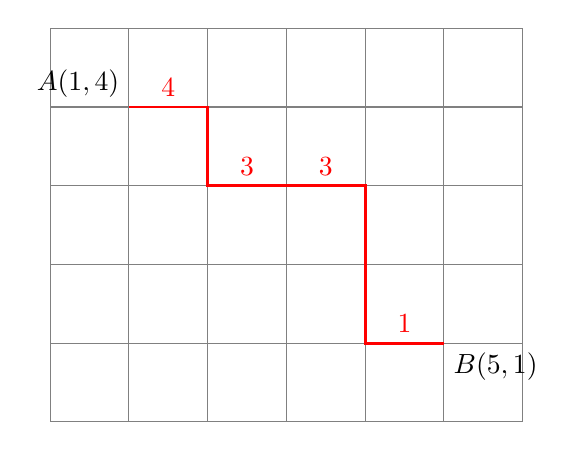
\begin{tikzpicture}
		\draw[step=1cm, color=gray] (0, 0) grid (6,5);
		\foreach \coord/\label [count=\xi] in {
			{1,4}/{$A(1,4)$},
			{5,1}/{$B(5,1)$}
		}{
		\pgfmathsetmacro\anch{\xi>1 ? "north west" : "south east"}
		\node[anchor=\anch] at (\coord) {\label};
		}
		\draw[line width=1pt, red] (1,4) -- node[above]{$4$} (2,4) -- (2,3) -- node[above]{$3$} (3,3) -- node[above]{$3$} (4,3) -- (4,1) -- node[above]{$1$} (5,1);
		\end{tikzpicture}
		\end{center}
	\end{fex}

	% ESEESSE from (1,4) to (5,1) example
	% x_1 x_3^2 x_4

	Clearly, this transformation is injective. This monomial $x_P$ has total degree $(\alpha - \beta)$ and only involves $x_i$ for $i \in [\delta,\gamma]$. As remarked, the set of all such monomials is in bijection with set of all paths. We encode the set of paths from $(\beta,\gamma)$ to $(\alpha,\delta)$ as the polynomial
	\[ h(\alpha-\beta,\delta,\gamma) = \sum_{\delta \le i_1 \le \cdots \le i_{\alpha-\beta} \le \gamma} x_{i_1} \cdots x_{i_{\alpha-\beta}}. \]
	Note that this is a variant of the complete homogenous polynomial we have seen.\\
	In more generality, we can have a \emph{path system} with $n$ pairs of points denoted by $\overline{\alpha} = (\alpha_1,\ldots,\alpha_n), \overline{\beta}, \overline{\gamma}, \overline{\delta}$ satisfying $\alpha_i \ge \beta_i$ and $\gamma_i \ge \delta_i$ for each $i$. Now, let us look at the set $NonIn(\overline{\alpha},\overline{\beta},\overline{\gamma},\overline{\delta})$ of non-intersecting (vertex-disjoint) paths $(P_1,\ldots,P_n)$, where $P_i$ is from $A_i = (\alpha_i,\gamma_i)$ to $B_i = (\beta_i,\delta_i)$. We encode each element of this set as the product of the polynomials of the constituent paths. Note that this can be used to recover the paths when the paths are non-intersecting.
	% maybe draw diagram for (1,2) to (2,1)
	
	% rewrite proof with transpose!
	\begin{ftheo}[Lindstr\"{o}m-Gessel-Viennot Lemma]
		Let $\NonIn(\pi(\overline{\alpha}),\overline{\beta},\overline{\delta},\pi(\overline{\gamma}))$ be non-empty only for $\pi = \Id$. Then,
		\[ \NonIn(\overline{\alpha},\overline{\beta},\overline{\gamma},\overline{\delta}) = \det M, \]
		where $M_{ij} = h(\alpha_j - \beta_i,\delta_j,\gamma_i)$, the set of paths from $A_i$ to $B_j$.
	\end{ftheo}
	\begin{proof}
		We would like to show that
		\[ \NonIn(\overline{\alpha},\overline{\beta},\overline{\gamma},\overline{\delta}) = \prod_{\pi \in \mathfrak{S}_n} \sign(\pi) \prod_{i=1}^n h(\alpha_{\pi(i)} - \beta_i , \delta_{\pi(i)} , \gamma_i). \]
		Suppose that according to some permutation $\pi$, some two paths from $A_i$ to $B_{\pi(i)}$ intersect. Consider the minimum intersecting pair index $(i,j)$ (according to the lexicographic order, say). Say the two paths intersect at $A$. Note that this cancels out with the set of paths for $(\pi(i), \pi(j)) \pi$ by looking at the paths from $A_i$ to $A$ to $B_{\pi(j)}$ and $A_j$ to $A$ to $B_{\pi(i)}$. Therefore, the only terms in the determinant that survive correspond to those $\pi$ which have non-intersecting paths, which is only $\Id$ by the hypothesis.
	\end{proof}

	\begin{ftheo}[Jacobi-Trudi Theorem]
		Let $\lambda \vdash d$ with $\lambda_1,\lambda_2,\ldots,\lambda_n$. Consider the $n \times n$ matrix $M_\lambda$ with $(M_\lambda)_{ij} = h_{\lambda_i + j -i}$, where $h_{n}$ is taken to be $0$ for negative $n$. Then, $s_\lambda = \det M_{\lambda}$.
	\end{ftheo}
	\begin{proof}
		Take some very large $N$ ($\infty$ in the limit). Consider the points $A_i = (n-i,N)$ and $B_i = (n-i+\lambda_i,1)$. In the limit as $N \to \infty$, the tranpose of the matrix from the previous question is \emph{precisely} $M_\lambda$! The set of paths from $A_j$ to $B_i$ is $h( (\lambda_i-i+n)-(n-j) , 1 , N ) = h_{\lambda_i + j - i}$.\\
		By the Lindstr\"{o}m-Gessel-Viennot lemma, the determinant of this matrix corresponds to the set of non-intersecting paths from $A_i$ to $B_i$ for each $i$ (it is easily checked that the only permutation with non-intersecting paths is the identity). To complete the proof, it suffices to establish an equivalence between such collections of paths and SSYTs of shape $\lambda$.\\
		Let us explain this bijection via an example.
		\begin{fex}
			Consider the partition $\lambda = (4,3,1)$ and set $N = 4$ for simplicity. The points are $A_1 = (2,4), A_2 = (1,4), A_3 = (0,4)$ and $B_1 = (6,1), B_2 = (4,1), B_3 = (1,1)$. Take the following collection of paths.

			\begin{center}
			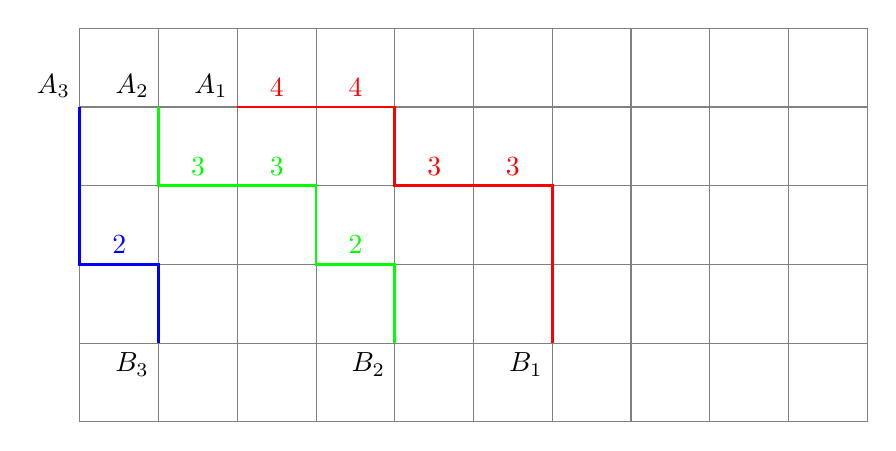
\begin{tikzpicture}
			\draw[step=1cm, color=gray] (0, 0) grid (10,5);
			\foreach \coord/\label [count=\xi] in {
				{2,4}/{$A_1$},
				{1,4}/{$A_2$},
				{0,4}/{$A_3$},
				{6,1}/{$B_1$},
				{4,1}/{$B_2$},
				{1,1}/{$B_3$}
			}{
			\pgfmathsetmacro\anch{\xi>3 ? "north east" : "south east"}
			\node[anchor=\anch] at (\coord) {\label};
			}
			\draw[line width=1pt, red] (2,4) -- node[above]{$4$} (3,4) -- node[above]{$4$} (4,4) -- (4,3) -- node[above]{$3$} (5,3) -- node[above]{$3$} (6,3) -- (6,1);
			\draw[line width=1pt, green] (1,4) -- (1,3) -- node[above]{$3$} (2,3) -- node[above]{$3$} (3,3) -- (3,2) -- node[above]{$2$} (4,2) -- (4,1);
			\draw[line width=1pt, blue] (0,4) -- (0,2) -- node[above]{$2$} (1,2) -- (1,1);
			\end{tikzpicture}
			\end{center}

			To this, we associate the tableau
			\[
			\begin{ytableau}
				4 & 4 & 3 & 3 \\
				3 & 3 & 2 \\
				2
			\end{ytableau}.
			\]
			Finally, to convert this to an SSYT, we replace each element with the maximum element in the tableau plus $1$ minus the element to get
			\[
			\begin{ytableau}
				1 & 1 & 2 & 2 \\
				2 & 2 & 3 \\
				3
			\end{ytableau}.
			\]
		\end{fex}
		It is evident that the shape of this SSYT is $\lambda$ and the rows are weakly increasing. So, it suffices to show that the columns are strictly increasing, that is, the columns of the earlier tableau are strictly decreasing. This means that if the $i$th east from $A_j$ to $B_j$ is taken at a height of $y$, then the $i$th east from $A_{j+1}$ to $B_{j+1}$ is taken at a height $y' < y$. By the definition of the paths, this path from $A_j$ to $B_j$ passes through $(n-j+i-1,y)$, and the path from $A_{j+1}$ to $B_{j+1}$ passes through $(n-(j+1)+i,y')$. Clearly, the sections of the two paths until here can be non-intersecting only if $y' < y$, completing the proof.
	\end{proof}

	% chapter 7 of stanley ec2
	% macdonald

	% littlewood-richardson coeffs
	% s_\lambda s_\mu = \sum_{\gamma \vdash \cdot} \alpha_{\lambda,\mu}^\gamma s_\gamma
	% what are the alpha? some alternating thing. has some relation to class functions of S_n. frobenius map (isometry from inner product to inner product) from class functions to degree n symmetric functions. irreducible characters go to schur symmetric functions!!!
	% because of this schur positivity becomes important